% Options for packages loaded elsewhere
\PassOptionsToPackage{unicode}{hyperref}
\PassOptionsToPackage{hyphens}{url}
%
\documentclass[
]{article}
\usepackage{amsmath,amssymb}
\usepackage{iftex}
\ifPDFTeX
  \usepackage[T1]{fontenc}
  \usepackage[utf8]{inputenc}
  \usepackage{textcomp} % provide euro and other symbols
\else % if luatex or xetex
  \usepackage{unicode-math} % this also loads fontspec
  \defaultfontfeatures{Scale=MatchLowercase}
  \defaultfontfeatures[\rmfamily]{Ligatures=TeX,Scale=1}
\fi
\usepackage{lmodern}
\ifPDFTeX\else
  % xetex/luatex font selection
\fi
% Use upquote if available, for straight quotes in verbatim environments
\IfFileExists{upquote.sty}{\usepackage{upquote}}{}
\IfFileExists{microtype.sty}{% use microtype if available
  \usepackage[]{microtype}
  \UseMicrotypeSet[protrusion]{basicmath} % disable protrusion for tt fonts
}{}
\makeatletter
\@ifundefined{KOMAClassName}{% if non-KOMA class
  \IfFileExists{parskip.sty}{%
    \usepackage{parskip}
  }{% else
    \setlength{\parindent}{0pt}
    \setlength{\parskip}{6pt plus 2pt minus 1pt}}
}{% if KOMA class
  \KOMAoptions{parskip=half}}
\makeatother
\usepackage{xcolor}
\usepackage[margin=1in]{geometry}
\usepackage{graphicx}
\makeatletter
\newsavebox\pandoc@box
\newcommand*\pandocbounded[1]{% scales image to fit in text height/width
  \sbox\pandoc@box{#1}%
  \Gscale@div\@tempa{\textheight}{\dimexpr\ht\pandoc@box+\dp\pandoc@box\relax}%
  \Gscale@div\@tempb{\linewidth}{\wd\pandoc@box}%
  \ifdim\@tempb\p@<\@tempa\p@\let\@tempa\@tempb\fi% select the smaller of both
  \ifdim\@tempa\p@<\p@\scalebox{\@tempa}{\usebox\pandoc@box}%
  \else\usebox{\pandoc@box}%
  \fi%
}
% Set default figure placement to htbp
\def\fps@figure{htbp}
\makeatother
\setlength{\emergencystretch}{3em} % prevent overfull lines
\providecommand{\tightlist}{%
  \setlength{\itemsep}{0pt}\setlength{\parskip}{0pt}}
\setcounter{secnumdepth}{-\maxdimen} % remove section numbering
% definitions for citeproc citations
\NewDocumentCommand\citeproctext{}{}
\NewDocumentCommand\citeproc{mm}{%
  \begingroup\def\citeproctext{#2}\cite{#1}\endgroup}
\makeatletter
 % allow citations to break across lines
 \let\@cite@ofmt\@firstofone
 % avoid brackets around text for \cite:
 \def\@biblabel#1{}
 \def\@cite#1#2{{#1\if@tempswa , #2\fi}}
\makeatother
\newlength{\cslhangindent}
\setlength{\cslhangindent}{1.5em}
\newlength{\csllabelwidth}
\setlength{\csllabelwidth}{3em}
\newenvironment{CSLReferences}[2] % #1 hanging-indent, #2 entry-spacing
 {\begin{list}{}{%
  \setlength{\itemindent}{0pt}
  \setlength{\leftmargin}{0pt}
  \setlength{\parsep}{0pt}
  % turn on hanging indent if param 1 is 1
  \ifodd #1
   \setlength{\leftmargin}{\cslhangindent}
   \setlength{\itemindent}{-1\cslhangindent}
  \fi
  % set entry spacing
  \setlength{\itemsep}{#2\baselineskip}}}
 {\end{list}}
\usepackage{calc}
\newcommand{\CSLBlock}[1]{\hfill\break\parbox[t]{\linewidth}{\strut\ignorespaces#1\strut}}
\newcommand{\CSLLeftMargin}[1]{\parbox[t]{\csllabelwidth}{\strut#1\strut}}
\newcommand{\CSLRightInline}[1]{\parbox[t]{\linewidth - \csllabelwidth}{\strut#1\strut}}
\newcommand{\CSLIndent}[1]{\hspace{\cslhangindent}#1}
\usepackage{setspace}
\usepackage[left]{lineno}
\usepackage{bookmark}
\IfFileExists{xurl.sty}{\usepackage{xurl}}{} % add URL line breaks if available
\urlstyle{same}
\hypersetup{
  pdftitle={Explicit Scale Simulation for analysis of RNA-sequencing count data with ALDEx2},
  hidelinks,
  pdfcreator={LaTeX via pandoc}}

\title{Explicit Scale Simulation for analysis of RNA-sequencing count
data with ALDEx2}
\author{true \and true \and true}
\date{}

\begin{document}
\maketitle
\begin{abstract}
In high-throughput sequencing (HTS) studies, sample-to-sample variation
in sequencing depth is driven by technical factors, and not by variation
in the scale (size) of the biological system. Typically a statistical
normalization removes unwanted technical variation in the data or the
parameters of the model to enable differential abundance analyses. We
recently showed that all normalizations make implicit assumptions about
the unmeasured system scale and that errors in these assumptions can
dramatically increase false positive and false negative rates. We
demonstrated that these errors can be mitigated by accounting for
uncertainty using a \emph{scale model}, which we integrated into the
ALDEx2 R package. This article provides new insights focusing on the
application to transcriptomic analysis. We provide transcriptomic case
studies demonstrating how scale models, rather than traditional
normalizations, can reduce false positive and false negative rates in
practice while enhancing the transparency and reproducibility of
analyses. These scale models replace the need for dual cutoff approaches
often used to address the disconnect between practical and statistical
significance. We demonstrate the utility of scale models built based on
known housekeeping genes in complex metatranscriptomic datasets. Thus
this work provides guidance on how to incorporate scale into
transcriptomic data sets.
\end{abstract}

\section{Introduction}\label{introduction}

\doublespacing \singlespacing 
\linenumbers

High-throughput sequencing (HTS) is a ubiquitous tool used to explore
many biological phenomenon such as gene expression (single-cell
sequencing, RNA-sequencing, meta-transcriptomics), microbial community
composition (16S rRNA gene sequencing, shotgun metagenomics) and
differential enzyme activity (selex, CRISPR killing). HTS proceeds by
taking a sample from the environment, making a library, multiplexing
(merging) multiple libraries together, and then applying a sample of the
multiplexed library to a flow cell. Each of these steps is a
compositional sampling step as only a fixed-size subsample of nucleic
acid is carried over to subsequent steps. Thus, with each sampling step
the connection between the actual number of molecules in the sampled DNA
pool and the environmental scale (e.g., total number of molecules,
microbial load, or total gene expression) of the measured biological
system is degraded or lost. In the end, the information contained in the
data relates only to relative abundances and has an arbitrary scale
imposed by the sequencing process (1--3).

The analysis of HTS data suffers from several known problems that can be
traced, in whole or in part, to misspecification of scale in the output
data. The first issue is poor control of the false discovery rate (FDR)
(4--8), exhibited as dataset-dependent FDR control which is observed as
a disconnect between statistical and biological significance (8, 9). In
current practice, this issue is addressed by a dual-filtering method,
whereby both a low p-value (or equivalently a low q-value following FDR
correction (10)) and a large difference between groups is used to
identify transcripts or genes of interest for follow-up analysis (9,
11). This double-filtering approach is graphically exemplified by the
volcano plot (11), but is known to not appropriately control the FDR
(12, 13). Since there is no standard way of determining what fold-change
cutoff should be used researchers have unlimited degrees of freedom
which is known to lead to unreliable inference (14). In particular Li et
al. (8) used patient or clinical-derived transcriptome datasets and
found that many methods suffer from an extremely high false positive
rate. The second issue is poor performance when analyzing data where the
mean change between groups is non-zero (3). Such asymmetric data can
arise when a gene set is expressed in one group but not the other, or
when one group contains different gene content from the other. This type
of data frequently arises in in-vitro selection experiments (SELEX),
transcriptome analysis, and microbiome analysis (15). The third issue is
that the actual scale of the environment is often a major confounding
variable during analysis (3, 16). This has long been known in
transcriptome analysis and was a major driver for the development of
normalization factors (17) and the use of molecular spike-ins to provide
a reference set of known counts (18--21) to estimate scale. While often
useful, spike-in methods only provide information downstream of the step
in the sample preparation protocol where the intervention was made and
introduce an additional source of variation that must be accounted for
(19). In the microbiome field, a recent landmark paper showed that
biological scale was a major unacknowledged confounder in many human
analyses (16). These authors built a machine learning model to uncover
the biological variation in scale and including this information was
useful despite exhibiting only a modest correlation (estimated to be
0.6) with the scale of data external to the training set (16). The final
issue is that all the above problems become more pronounced as more
samples are collected; that is, more information results in optimizing
for a precise but inaccurate analysis (3, 8, 22).

The four problems were recently shown by Nixon et al. (3) to be a result
of a mismatch between the underlying size or scale of the system and the
assumptions of the normalizations used for the analysis of HTS.
Biological variation in scale often represents an important unmeasured
confounder in HTS analyses (15, 16, 19, 23). For example, cells
transformed by the cMyc oncogene have about 3 times the amount of mRNA
and about twice the rRNA content than non-transformed cells (24), and
this dramatically skews transcriptome analysis unless spike-in
approaches are used (19). In addition, wild-type and mutant strains of
cell lines, yeast or bacteria have different growth rates and RNA
contents under different conditions, which affect our ability to
identify truly differentially abundant genes (25--27). As another
example, the total bacterial load of the vaginal microbiome differs by
1-2 orders of magnitude in absolute abundance between the healthy and
bacterial vaginosis states (28), and the cell and RNA composition
between these states is dramatically different (29, 30). Thus, a full
description of any of these systems includes both relative change
(composition) and absolute abundance (scale). Current methods access
only the compositional information yet make implicit assumptions about
the scale (22).

Nixon et al. (3) showed that the challenge of non-biological variation
in sequencing depth could be explained as a problem of
partially-identified models. They showed that \emph{all} normalizations
make some assumption about scale but these implicit assumptions are
often inappropriate and difficult to interpret. As a result, different
normalizations provide different outputs when applied to the same
dataset (4, 6, 17, 31, 32). Intuitively, normalizations in widespread
use assume that either all samples have the same scale,
e.g.~proportions, rarefaction (33), RPKM (34, 35), etc; or that a subset
of features in one sample can be chosen as a reference to which the
others are scaled e.g.~the TMM (36), the LVHA (15) qPCR (37), the
additive log-ratio (38); or that different sub-parts of each sample
maintain a constant scale across samples e.g.~the RLE (39); or that the
geometric mean of the parts is appropriate e.g the CLR (40) and its
derivatives. Notably when the assumption of similar scale across samples
is not violated, or violated only weakly, any method will provide a
reasonable analysis. The problem arises when this assumption is
violated, in which case all tools fail without warning.

\begin{figure}

{\centering 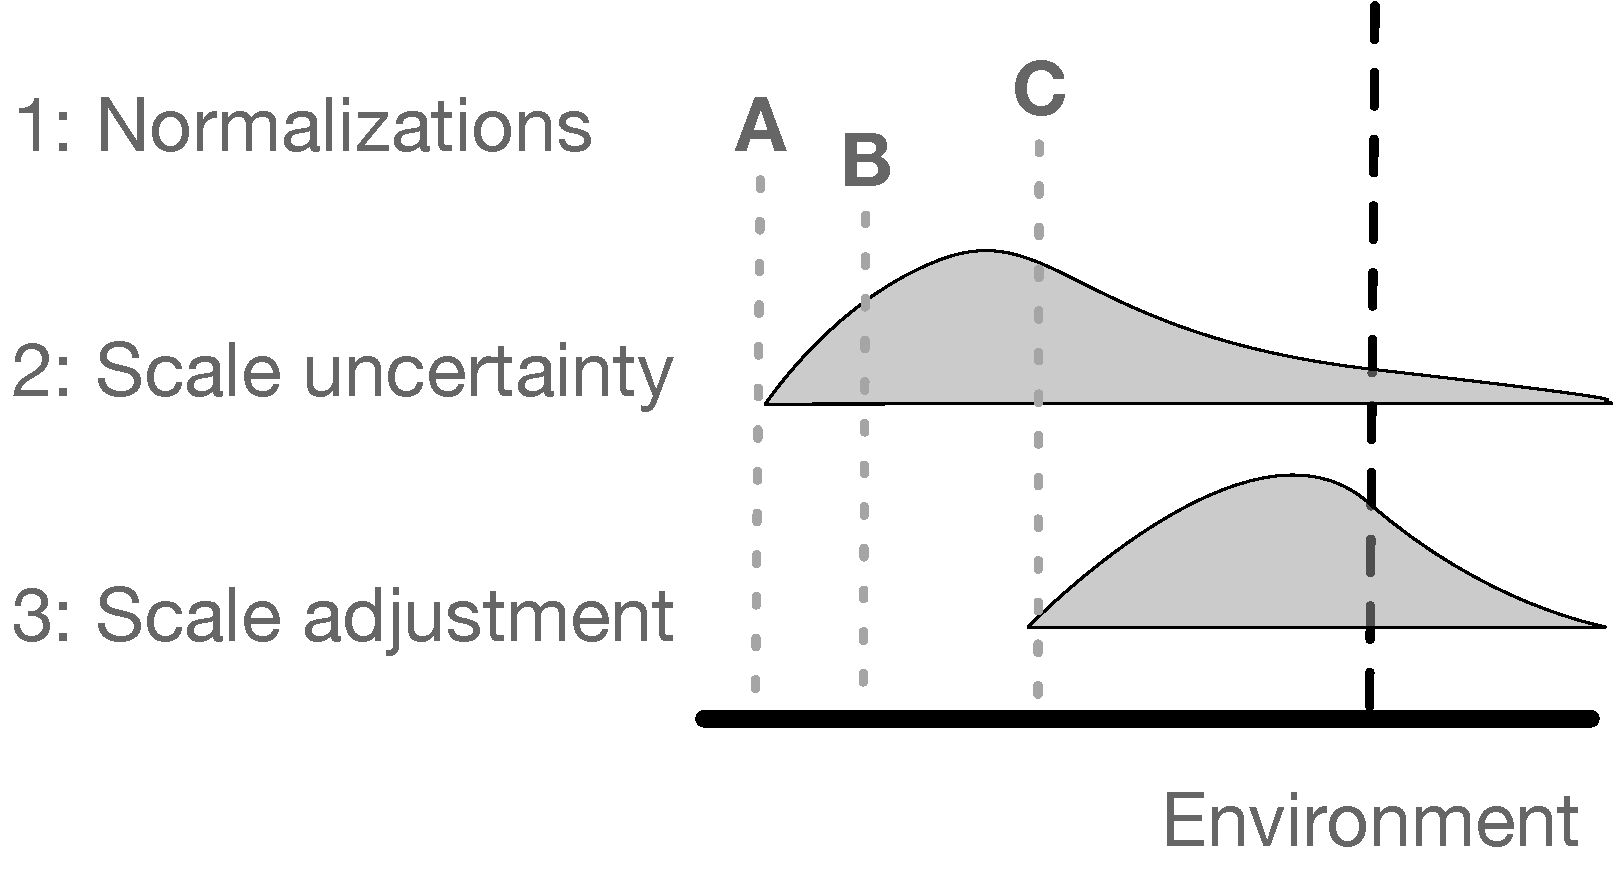
\includegraphics[width=0.6\linewidth]{./go3_files/figure-latex/scale-explained} 

}

\caption{Mismatches between estimated scale and true scale lead to poor estimation of high throughput sequencing data. All normalizations used for differential abundance analysis make some strict assumption about the scale of the environment as shown in line 1. In this example all normalizations produce a biased estimate of the environmental scale, but estimate C is the closest to the truth.  Adding uncertainty to normalization C as represented by the distribution in the line 2 leads to less bias and now includes the actual environmental scale in the assumption. As shown in line 3 in some cases it may be useful to adjust the centre of the scale uncertainty estimate if the initial normalizations give very poor estimates of the underlying environment.}\label{fig:unnamed-chunk-1}
\end{figure}

The original scale-naive ALDEx2 (41) model unwittingly made a strict
assumption about scale through the CLR normalization and we found that
the CLR was very sensitive to violations of the assumption of scale
identity between groups (15). Moreover, when the assumption of identity
was not true the CLR used by ALDEx2 could be outperformed by other
normalizations in simulation studies (42). As illustrated graphically in
Figure 1, Nixon et al. (3) showed through simulation that introducing
uncertainty in the scale assumptions, and in extreme cases altering the
location of the scale assumption, resulted in more reproducible data
analysis including better control of both false positive and false
negative results. We modified ALDEx2 to explicitly model uncertainty in
scale over a range of reasonable normalization parameters, and showed
significant improvements in performance in microbiome and in-vitro
selection experiments (22) and in a vaginal metatranscriptome analysis
(43). Here, we briefly review these modifications and show how adding
scale uncertainty can greatly improve modeling in transcriptome and
meta-transcriptome datasets to provide substantially more robust and
reproducible results.

\section{Implementation}\label{implementation}

Formal and expanded descriptions of the concepts that follow are given
in (3, 22). To be concrete, we let \(\mathbf{Y}\) denote the
\emph{measured} \(D \times N\) matrix of sequence counts with elements
\(\mathbf{Y}_{dn}\) indicating the number of measured DNA molecules
mapping to feature \(d\) (e.g., a taxon, transcript or gene) in sample
\(n\). Likewise, we can denote \(\mathbf{W}_{dn}\) as the \emph{true}
amount of class \(d\) in the biological system from which sample \(n\)
was obtained. We can think of \(\mathbf{W}\) as consisting of two parts,
the scale \(\mathbf{W}^{Tot}\) (e.g., totals) and the composition
\(\mathbf{W}^{Comp}\) (i.e., proportions). That is, \(\mathbf{W}^{Tot}\)
is a \(N\)-vector with elements
\(\mathbf{W}^{Tot}_{n}=\sum_{d}\mathbf{W}_{dn}\) while
\(\mathbf{W}^{Comp}\) is a \(D \times N\) matrix with elements
\(\mathbf{W}^{Comp}_{dn}=\mathbf{W}_{dn}/\mathbf{W}^{Tot}_{n}\). Note
that with these definitions \(\mathbf{W}\) can be written as the
element-wise combination of scale and composition:
\(\mathbf{W}_{dn}=\mathbf{W}^{Comp}_{dn}\mathbf{W}^{Tot}_{n}\), or as
the logarithm
\(\log \mathbf{W}_{dn}= \log \mathbf{W}^{Comp}_{dn} + \log \mathbf{W}^{Tot}_{n}\).

Many of the normalizations used in tools such as DESeq2 (44), edgeR
(36), metagenomeSeq (45) ALDEx2 (46) can be stated as ratios of the form
\(\hat{{\mathbf{W}}}_{dn} \approx \mathbf{Y}_{dn}/f(\mathbf{Y})\), where
the denominator is determined by some function of the observation. We
use the hat notation (\(\ \hat{}\ \)) to indicate that the output is an
estimate of the true value. The technical variation in sequencing depth,
which is often called ``library size'' has no relationship with the
actual number of molecules in the sampled environment (1). In other
words (\(\mathbf{Y}^{Tot}_{n}=\sum_{d}\mathbf{Y}_{dn}\)) the observed
data \(\mathbf{Y}\) provides us with information about the system
composition \(\mathbf{W}^{Comp}\) but little to no information in the
system scale \(\mathbf{W}^{Tot}\) (Lovell et al.~2011).

\subsection{Adding Scale Uncertainty in
ALDEx2}\label{adding-scale-uncertainty-in-aldex2}

The ALDEx2 R package (41, 46) is a general purpose toolbox to model the
uncertainty of HTS data and to use that model to estimate the
significance of the underlying LFC (log-fold change). At a high-level,
ALDEx2 has three connected components to estimate the uncertainty
inherent in HTS datasets. First, the tool accounts for the uncertainty
of the sequencing counts using Dirichlet multinomial sampling to build a
probabilistic model of the data; i.e.,
\(\mathbf{\hat{W}}^{Comp} \approx \mathrm{Dir}(\mathbf{Y})\). Secondly,
ALDEx2 uses the centred log-ratio transformation to scale the data (41).
It was this step that was modified to account for scale uncertainty and
misspecification (22) explained with more details in (3, 22) and
summarized in the next paragraph. Finally, a standard null-hypothesis
test and a non-parametric estimate of mean standardized difference are
used to report on the finite sample variation. These sources of
uncertainty and variation are combined via reporting the expected values
from a Monte-Carlo simulation framework. For simplicity, we use the term
`difference' to refer to the absolute difference between groups, and
`dispersion' to refer to the within-condition difference or pooled
variance as defined in (41). These are calculated on a \(\log_2\) scale.
For more details on ALDEx2 see (3, 22, 41, 46).

Scale models were incorporated into ALDEx2, turning the ALDEx2 model
into a specialized type of statistical model which Nixon et al. (3) term
a \textit{Scale Simulation Random   Variable} (SSRV). To do this, Nixon
et al. (3) generalized the concept of normalizations by introducing the
concept of a \textit{scale model} to account for potential error in the
centred log-ratio normalization step. They did this by including a model
for \(\mathbf{\hat{W}}^{Tot}_{n}\). The CLR normalization used by ALDEx2
makes the assumption \(\mathbf{\hat{W}}^{Tot}_{n}=1/G_{n}\), where
\(G_n\) is the geometric mean of the counts (or the corresponding
proportions)of each part in sample n, which while being a random
variable, is essentially constant across each Monte-Carlo replicate, but
that differs between samples. With this modification, ALDEx2 can be
generalized by considering probability models for the scale
\(\mathbf{\hat{W}}^{Tot}_{n}\) that have mean \(1/G_{n}\). For example,
the following scale model generalizes the CLR:

\[\log \mathbf{\hat{W}}^{Tot}_{n} = -\log G_{n} + \Lambda x_{n} \qquad \Lambda \sim N(\mu, \gamma^{2}).\]

This formulation is quite flexible (3, 22). In the simple or `default'
configuration, \(\mu = 0\) and \(\gamma\) is a tunable parameter drawn
from a log-Normal distribution (3). Adding scale uncertainty with the
\(\gamma\) paramenter (as shown in Figure 1:1) controls only the degree
of uncertainty of the CLR assumption for the \(x_{n}\) binary condition
indicator (e.g., \(x_{n}=1\) denotes case and \(x_{n}=0\) denotes
control). In the advanced or `informed' configuration, \(\mu\) takes
different values for each group and controls the location of the LFC
assumption (as shown in Figure 1:2); combining \(\mu\) with a \(\gamma\)
estimate allows for uncertainty in both the location and the scale. In
the manuscript where the idea of scale was original derived, Nixon et
al. (3) conducted extensive simulations showing that both the default
and informed approaches exhibit increased sensitivity and specificity
(22). In this report we show that these approaches also work well to
control the FDR in transcriptome and metatranscriptome datasets. We also
provide some additional insights into how this is achieved. These
modifications are instantiated in ALDEx2 which is the first software
package designed for SSRV-based inference.

\section{Results}\label{results}

\subsection{Adding scale uncertainty replaces the need for dual
significance
cutoffs.}\label{adding-scale-uncertainty-replaces-the-need-for-dual-significance-cutoffs.}

Gierliński et al. (47) generated a highly replicated yeast transcriptome
dataset to compare gene expression between a wild-type strain and a snf2
gene knockout, \(\Delta\)snf2. This dataset of 86 samples (44 and 42 per
group) is an example of technical growth replicate experiments common in
the literature. The dataset was used to test several RNA-seq tools for
their power to detect the set of differentially abundant transcripts
identified in the full dataset when the data was subset (9). In this
original study each tool had its own `gold standard' set of transcripts
with different tools identifying between between 65\% to
\textgreater80\% of all transcripts as being significantly different.
Since the majority of transcripts were significantly different, the
authors suggested that it was more appropriate to apply a dual cutoff
composed of both a Benjamini-Hochberg (48) corrected p-value (q-value)
plus a difference cutoff to limit the number of identified transcripts
to a much smaller fraction of the total. In other datasets, Nixon et al,
(22) showed that adding even a small amount of scale uncertainty with
ALDEx2 dramatically reduced the number of significant transcripts
identified, removing the need for the dual cutoff approach in this
dataset and others.

\begin{figure}

{\centering 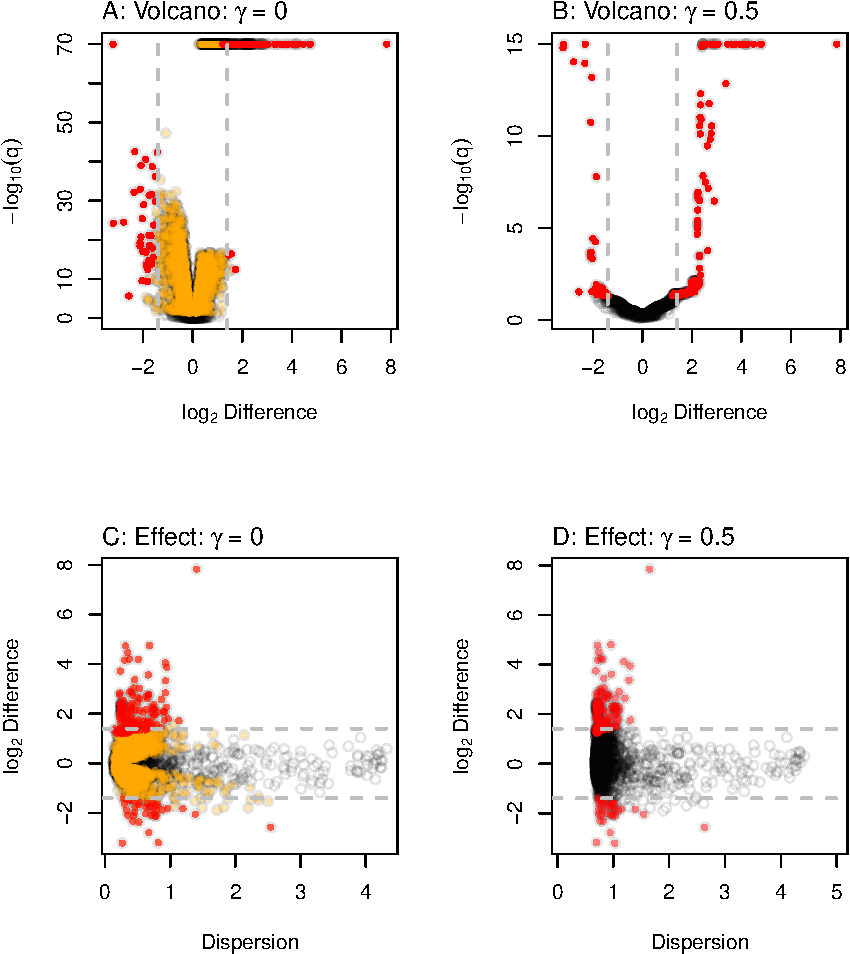
\includegraphics[width=0.8\linewidth]{go3_files/figure-latex/yst-plot-1} 

}

\caption{Volcano and effect plots for unscaled and scaled transcriptome analysis. ALDEx2 was used to conduct a differential expression (DE) analysis on the yeast transcriptome dataset. The results were plotted to show the relationship between difference and dispersion using effect plots or difference and the q-values using volcano plots. Panels A,C are for the naive analyses, and Panels B,D are for the  default analyses that include scale uncertainty. Each point represents the values for one transcript, with the color indicating if that transcript was significant in the both analyses (red) or in the naive analysis only (orange). Points in grey are not statistically signficantly different under any condition. The horizontal dashed lines represent a \(\log_2\)difference of \(\pm 1.4\).}\label{fig:yst-plot}
\end{figure}

We start with the assumption that not all statistically significant
differences are biologically relevant (49), and that a result where the
majority of transcripts are significant breaks the necessary assumption
for DA/DE expression that most parts be invariant (31). Transcriptomic
analysis commonly uses a dual cutoff approach graphically exemplified by
volcano plots (9, 11). Using either DESeq2 or ALDEx2, a majority of
transcripts are statistically significantly different between groups
with a q-value cutoff of \(\le 0.05\); i.e.~4636 (79\%, DESeq2) or 4172
(71\%, ALDEx2) of the 5891 transcripts. These values are in line with
those observed by (9). Such large numbers of statistically significant
transcripts seems biologically unrealistic. That 118 transcripts are
identified by ALDEx2 and not DESeq2, while DESeq2 identifies 582
transcripts that ALDEx2 does not, suggests that the choice of
normalization plays a role in which results are returned as significant
and that some, if not the majority, are driven by technical differences
in the analysis (8, 31) or are false positives.

The Volcano plots in Figure 2 A and B show that adding scale uncertainty
increases the minimum q-value and increases the concordance between the
q-value and the difference between groups (compare panels A and B). The
effect plots (50) in Figure 2C shows that the majority of significant
transcripts (red, orange) have negligible differences between groups and
very low dispersion. We suggest that this low dispersion is driven by
the experimental design which is actually a technical wet lab
replication rather than a true biological replication design (47). Scale
uncertainty can be incorporated using the \texttt{gamma} parameter that
controls the amount of noise added to the CLR mean assumption when we
call either \texttt{aldex()}, or \texttt{aldex.clr()}. Figure 2 B,D
shows that setting \(\gamma=0.5\) now results in 205 which is far fewer
statistically significant transcripts than in the naive analysis and we
observe that the minimum dispersion increases from 0.12 (\(\gamma = 0\)
) to 0.67 (\(\gamma=0.5\)).

It is common practice to use a dual-cutoff by choosing transcripts based
on a thresholds for both q-values and fold-changes (9), and these were
first proposed for microarray experiments through volcano plots (11).
Note that there is considerable variation in recommended cutoff values
(9), and that this controversy has persisted ever since fold-change was
suggested (51). Unfortunately, universal cutoff fold-change values
cannot be identified in part because different tools have intrinsically
different variance in their log\_2-fold change ranges (52). This has led
to the widespread practice of applying a post-hoc fold-change cutoff to
reduce the number of positive identifications to a manageable proportion
of the whole dataset. Here, we applied the dual-cutoff method using a
fold-change of at least a \(2^{1.4}\) fold change that reduces the
number of significant outputs to 193 for DESeq2 and to 186 for ALDEx2.
This cutoff was chosen for convenience and is mid-way between the high
and low fold-change recommendations of (9). These limits are shown by
the dashed grey lines in Figure 2 and we can see that a \(2^{1.4}\) fold
change \((\sim 2.6\) fold) cutoff identifies a similar number of
transcripts as does ALDEx2 using \(\gamma = 0.5\) which identifies 205
transcripts.

Supplementary Figures 1 shows an example of the
\texttt{aldex.senAnalysis()} function to identify those transcripts that
are very sensitive to scale uncertainty in this dataset. Here we see
that adding a very small amount of scale \(\gamma = 0.1\) reduces the
number of significant transcripts by more than half in the yeast
dataset. This allows the analyst to ignore those low-dispersion
transcripts that were significant only because of an absence of scale
uncertainty.

We next examined how adding scale would alter the analysis in a real
dataset to which synthetically generated true positive counts had been
added. We show results from the anti-PD-1 therapy RNA-seq dataset (53)
which examined changes in gene expression when cells were exposed or not
to a cell-cycle checkpoint inhibitor. This dataset was used by Li et al.
(8) as an example of the dangers of relying on tools with high false
positive error rates when analyzing clinical or clinically-related
transcriptome samples. Indeed, in the benchmarking analysis done by this
group, they found that parameter based methods such as DESeq2 and edgeR
that on reported p-value and fold-change cutoffs often led to
conclusions in the original dataset that were indistinguishable from
permutations of the dataset. In other words, that the analysis of
transcriptome datasets from patient-derived samples often exhibited many
false-positive identifications.

\begin{figure}

{\centering 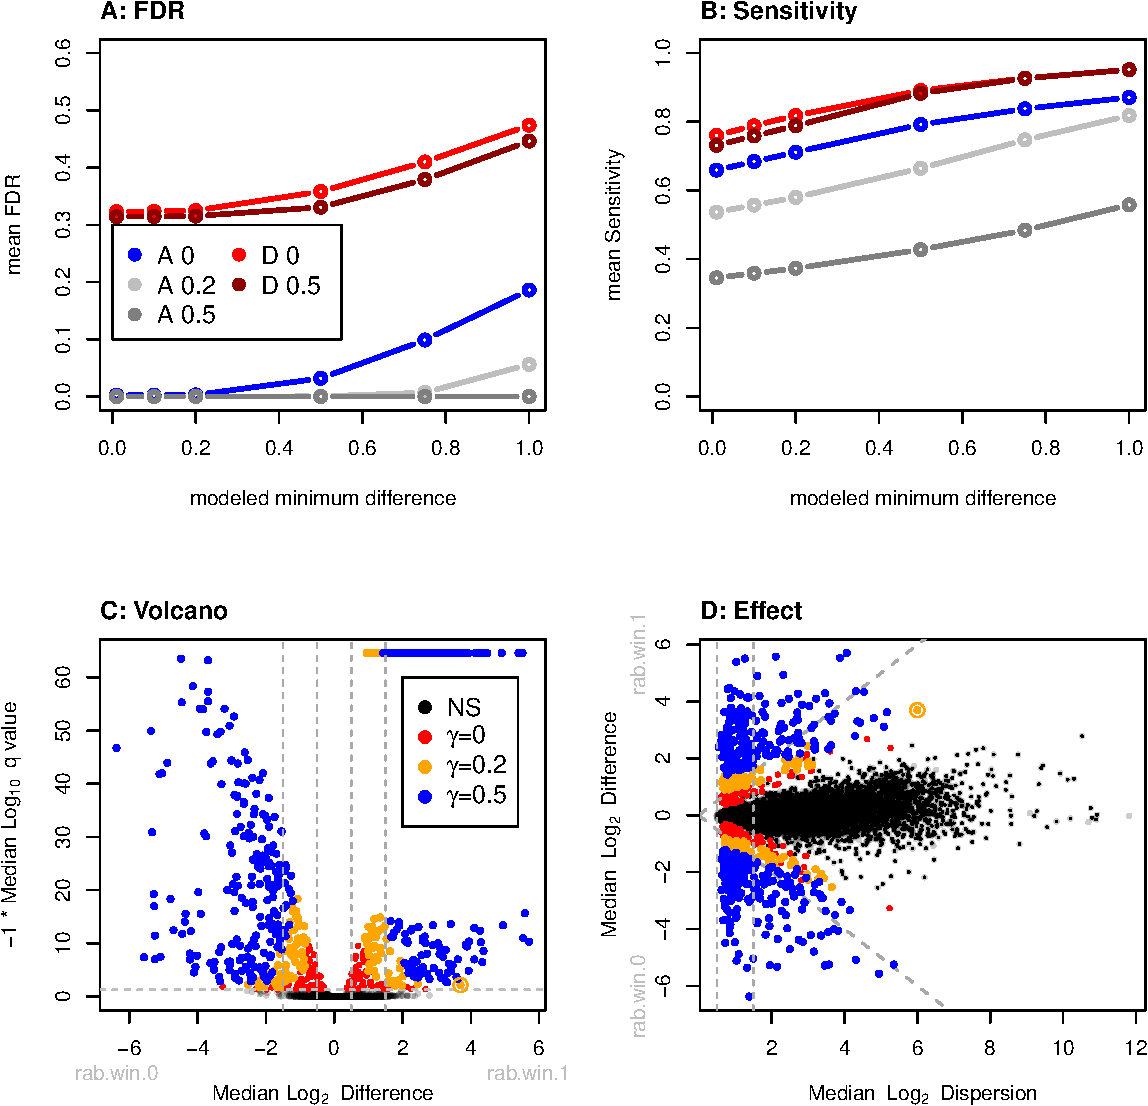
\includegraphics[width=0.8\linewidth]{go3_files/figure-latex/immuno-1} 

}

\caption{Results of modeling true positive (TP) differences in the PD-1 dataset. For this the data were shuffled and  5\% of the transcripts were modeled to have TP differences between groups where the differences were drawn from a Normal distribution with a mean difference of 0 and a sd of 2. Panel A shows the mean FDR of 10 instances for scale-naive ALDEx2 (A 0), and ALDEx2 with \(\gamma=0.2\) (A 0.2) or \(\gamma=0.2\) (A 0.5), and where significant features were identified by  DESeq2 without (D 0), or with (D 0.5) a 0.5-fold change difference. The x-axis shows how the FDR changes for each tool as a function of the estimated modeled difference between groups. Panel B shows the mean sensitivity (TP found /all TP). Panels C and D show volcano and effect plots for the ALDEx2 output with the transcripts identified as significant at each scale setting as colored points, and non-significant transcripts in black.}\label{fig:immuno}
\end{figure}

Figure 3 shows the results of ten permutations of this dataset while
simulating 5\% of the transcripts to be true positives where the
difference from no change was derived from a Normal distribution (54).
This simulation was conducted with the \texttt{seqgendiff} R package
(54) to both permute the dataset and to add true positive features. We
did ten permutations and kept track of the number of true and false
positive identifications. Figure 3A shows the actual false discovery
rate for ALDEx2 with and without the addition of scale uncertainty and
for DESeq2 with or without a fold-change cutoff of \(2^{0.5}\). When the
modeled difference was greater than 0, ALDEx2 exhibited a FDR of
\(\gamma = 0\): 0.002, \(\gamma = 0.2\): 0, and \(\gamma = 0.5\): 0,
while DESeq2 with no fold-change cutoff had an FDR of 0.32 and with a
0.5 fold-change cutoff an FDR of 0.31. Figure 3 also plots these results
as a function of the minimum modelled fold change of the true positive
transcripts. First, we can see that this analysis recapitulates the
observations of Li et al (8) in that DESeq2 has very poor false positive
control at a nominal FDR of 0.05. The FDR is not controlled any better
when a fold-change cutoff is applied, and this agrees with previous work
showing that fold-change cutoffs do not materially improve FDR control
in high throughput datasets (12, 13). Figure 3B shows that DESeq2 has
higher sensitivity than does ALDEx2, and not surprisingly this
sensitivity increases as the difference between groups increases. For
the case where the mean difference is 0 or greater, ALDEx2 exhibited a
sensitivity of \(\gamma = 0\): 0.66, \(\gamma = 0.2\): 0.54, and
\(\gamma = 0.5\): 0.35, while DESeq2 with no fold-change cutoff had a
sensitivity of 0.76 and with a 0.5 fold-change cutoff a sensitivity of
0.73. In this example, scale-naive ALDEx2 has near perfect FDR control
and reasonable sensitivity at low modeled difference between groups.
However, when the modeled difference between groups becomes large, then
the scale-naive version of ALDEx2 begins to exhibit unacceptable rates
of false positives and the false positive rate for DESeq2 also
increases. Adding in even small amounts of scale uncertainty drops the
true FDR rate to 0, but at the expense of sensitivity. The major
contributor to the increase in FDR with larger modeled differences is
that the tools are identifying as positives those transcripts that are
modeled to have differences just below the threshold. We need to
recognize that there is no such thing as a statistical free lunch; the
analyst can have high sensitivity but low confidence that any individual
transcript is truly different, or have lower sensitivity but have very
high confidence that the difference is real. In other words, the
sensitivity of a method is directly tied to how much error the
investigator is willing to tolerate.

Examination of the volcano plot (11) and effect plot (50) in Figure 3C
and D provides some insight into why adding scale uncertainty provides
better FDR control than does the approach of using a p-value and a
fold-change cutoff. In the volcano plot, adding scale uncertainty
differentially excludes transcripts with a combination of marginal
p-values and low difference between groups, and that this becomes more
pronounced with a larger scale value. This effect is also seen in Figure
2 but is more nuanced. In contrast, the fold-change cutoff does not
incorporate the magnitude of the p-value and so transcripts with large
differences, but marginal p-values are retained. The effect plot in
Figure 3D shows that the transcripts with marginal p values and large
differences that are excluded when scale uncertainty is added are those
that have a large dispersion.

As a concrete example consider the point that is circled in panels C and
D with a marginal p-value, with a difference between of nearly 4 and a
dispersion of greater than 6. This transcript is no longer significant
when \(\gamma = 0.2\), but would require a very large fold-change cutoff
to be excluded by the standard approach. In addition, transcripts with
very small dispersion and very small differences are also excluded when
scale uncertainty is added. Thus, the addition of scale uncertainty
achieves the desired outcome of lowering the FDR for those transcripts
that are either marginally differentially abundant, or where the
underlying dispersion--and hence the uncertainty in measurement--is very
high, or for transcripts that fit both criteria.

Supplementary Figure 2 shows a second permuted dataset with the addition
of modeled differences between groups. Here we used another real dataset
with over 200 biological replicates of BRCA1 tumor and control tissue
samples from Li et al. (8). This Supplementary Figure shows that the FDR
control of DESeq2 is somewhat better than in the PD-1 dataset, although
still much greater than the the anticipated 5\%. Further, a fold-change
cutoff reduces the FDR of DESeq2 from about 30\% to just over 20\% with
a power of over 80\%. However, we can see that scale-naive ALDEx2
performs substantially better with a negligible FDR and comparable
power. Adding scale uncertainty again improves FDR even for those
transcripts modeled to have larger differences and the power is
substantially better than in the PD-1 dataset, reaching the same power
as DESeq2 or scale-naive ALDEx2 when the modeled difference is large. As
before, this is driven by removing from consideration those transcripts
with either a small difference between or a marginal p-value, or both.

Supplementary Figures 3 shows that effect of applying \(\gamma = 0.5\)
to this dataset results in reducing the number of positive transcripts
from being \(\sim 70\)\% of the whole dataset to less than 10\% of the
dataset and that this is largely because of a reduction in significance
of those transcripts with low dispersion. Supplementary Figures 4 shows
a sensitivity analysis of the BRCA1 dataset showing that different scale
uncertainty amounts alter the number of significant transcripts in a
biological replicate experiment similarly to a technical replicate
experiment. Supplementary Figures 5 and 6 delve into how adding scale
uncertainty affects the variace-abundance relationship in subtle ways,
and may help readers to understand the observations seen in Figure 3 and
supplementary Figure 2.

Together the results in this section show that adding scale uncertainty
has the desirable effect of altering the transcripts identified as
significantly different between groups in a way that exhibits better
control of FDR albeit with a corresponding reduction in sensitivity.
Those parts that were statistically significantly different \emph{only
because of low dispersion} or that \emph{had marginal p-values} or both,
are now preferentially excluded from statistical significance. In
practice, we suggest that a \texttt{gamma} parameter of between 0.2 and
0.5 is realistic for most experimental designs (22) regardless if the
replication is technical or biological.

\subsection{Housekeeping genes and functions to guide scale model
choices.}\label{housekeeping-genes-and-functions-to-guide-scale-model-choices.}

Dos Santos et al. (55) used a vaginal metatranscriptome dataset to
compare the gene expression in bacteria collected from healthy (H) and
bacterial vaginosis (BV) affected women. This dataset is derived from
two publicly available datasets composed of a set of 20 non-pregnant
women from London, Ontario Canada (56) and a subset of 22 non-pregnant
women collected from German women who underwent metronidazole treatment
for BV (57). Batch effects for these two groups were removed with
ComBat-seq (58) and the two datasets were merged into one, giving a
total of 16 H and 26 BV samples. In the Dos Santos paper, all results
from this initial analysis were replicated in a much larger dataset
derived from the MOMS-PI study (59)

In this vaginal environment, both the relative abundance of species
between groups and the gene expression level within a species is
different (60). Additionally, prior research suggests that the total
number of bacteria is about 10 times more in the BV than in the H
condition (28). Thus, these are extremely challenging datasets in which
to determine differential abundance as there are both compositional and
scale changes between conditions. The usual method to analyze vaginal
metratranscriptome data is to do so on an organism-by-organism basis
(57, 59, 60) because the scale confounding of the environment is less
pronounced. One attempt at system-wide analysis returned several
housekeeping functions as differentially expressed between groups (57);
a result likely due to a disconnect between the assumptions of the
normalization used and the actual scale of the environment (15).

\begin{figure}
\centering
\pandocbounded{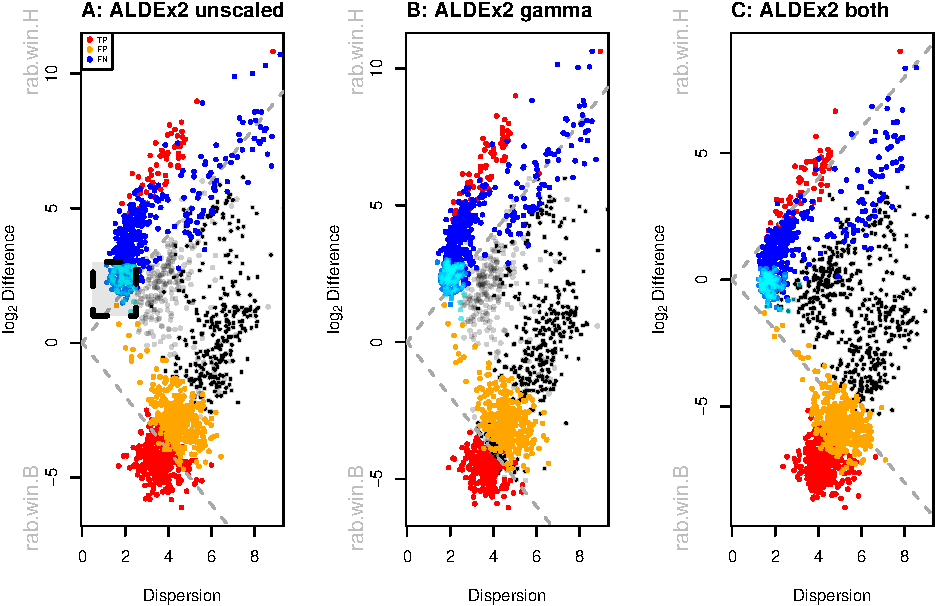
\includegraphics[keepaspectratio]{go3_files/figure-latex/meta-1.pdf}}
\caption{Analysis of vaginal transcriptome data aggregated at the Kegg
Orthology (KO) functional level. Panel A shows an effect plot for the
default analysis where the functions that are elevated in the healthy
individuals have positive values and functions that are elevated in BV
have negative values. Highlighed in the box are KOs that are almost
exlusively housekeeping functions; these and are colored cyan. These
housekeeping functions should be located on the midline of no
difference. Panel B shows the same data scaled with \(\gamma = 0.5\),
which increase the minimum dispersion as before. Panel C shows the same
data scaled with \(\gamma = 0.5\) and a 0.14 fold difference in
dispersion applied to the BV samples relative to the H samples. In these
plots statistically significant (q-value \textless{} 0.01) functions in
the informed model are in red, false positive functions are in blue,
non-significant functions in black and false negative functions are in
orange.}
\end{figure}

In this example, we show how to specify and interpret a user defined or
\emph{informed} scale model that can explicitly account for some of
these modeling difficulties (22) even in a difficult to analyze dataset.
An informed scale model can control for both the mean difference of
scale between groups (e.g., directly incorporate information on the
differences in total number of bacteria between the BV and H conditions)
as well as the uncertainty of that difference as illustrated in Figure
1:3. To specify a user-defined scale model, we can pass a matrix of
scale values instead of an estimate of just the scale uncertainty to
\texttt{aldex.clr()}. This matrix should have the same number of rows as
the of Monte-Carlo Dirichlet samples, and the same number of columns as
the number of samples. While this matrix can be computed from scratch by
the analyst, there is an \texttt{aldex.makeScaleModel()} function that
can be used to simplify this step in most cases. This encodes the scale
model as \(\Lambda \sim N(log_2 \mu_n, \gamma^{2})\), where \(\mu_n\)
represents the scale value for each sample or group and \(gamma\) is the
uncertainty as before. The scale estimate can be a measured value (cell
count, nucleic acid input, spike-ins, etc) or an estimate. Nixon et al.
(3, 22) showed that only the ratio of the means are important when
providing values for \(\mu_n\); i.e., the ratio between the
\(\log_2 \mu_i\) and \(\log_2 \mu_j\) values. See the supplement to
Nixon et al. (22) for more information.

Figure 4A shows an effect plot of the data where reads are grouped by
homologous function regardless of the organism of origin. Each point
represents one of 3728 KEGG functions (61). There are many more
functions represented in the BV group (bottom) than in the healthy group
(top). This is because the \textit{Lactobacilli} that dominate a healthy
vaginal microbiome have reduced genome content relative to the anaerobic
organisms that dominate in BV, because there is a greater diversity of
organisms in BV than in H samples, and because the BV condition has
about an order of magnitude more bacteria than does the H condition.

The naive scale model appears to be reflecting the bacterial load as
observed by calculating the mean scale value for each group. Using a
negligible scale value; i.e., \(\gamma=1e-3\) exposes the naive scale
estimate for samples in the \texttt{@scaleSamps} slot from the
\texttt{aldex.clr} output. The naive scale estimate for the healthy
group is 17.41 and for the BV group is 14.59 for a difference of 2.82.
This is interpreted as the scale of the H group of samples being 7.06
greater than the BV group.

Applying the default scale model of \(\gamma=0.5\) increases the
dispersion slightly but does not move the housekeeping functions toward
the midline. This is as expected; the mean of the default scale model is
based on the CLR normalization so no shift in location would be expected
over the scale-naive ALDEx2 model. Nevertheless, about 30\% of the
housekeeping functions are no longer statistically significantly
different. Note that this change is simple to conduct, has no additional
computational complexity and requires only a slight modification for the
analyst.

There are 101 functions with low dispersion that appear to be shared by
both groups (boxed area in Figure 3A, and colored in cyan). Inspection
shows that these largely correspond to core metabolic functions such as
transcription, translation, ribosomal functions, glycolysis,
replication, chaperones, etc (Supplementary file housekeeping.txt). The
transcripts of many of these are commonly used as invariant reference
sequences in wet lab experiments (62) and so are not be expected to
contribute to differences in ecosystem behaviour. Because we expect
housekeeping functions to be nearly invariant in their expression and to
occur in all organisms, the average location of these should be centred
on 0 difference to represent an internal reference set. However, with
the naive scale model, the mean of these housekeeping functions is
approximately located at 2.3. Thus, we desire a scale model that
approximately centres the housekeeping functions and an appropriate
scale in this dataset for functional analysis will place these functions
closer to 0 than does the naive estimate. One way to choose an
appropriate value for \(\mu_n\) is to use the \texttt{aldex.clr}
function on only the presumed invariant functions setting
\(\gamma > 0\), and then accessing the \texttt{@scaleSamps} slot as
before. Doing so suggests that the difference in scale should be about
14\%. A second approach would be to identify the functions used as the
denominator with the \texttt{denom="lvha"} option (15) for the
\texttt{aldex.clr} function, and then to use these values as before.
This approach suggests a 5\% difference in scale, and is potentially
less subject to user interpretation.

For the purposes of this example, if we assume a 14\% difference in
scale, we can set \(\mu_i = 1\) and \(\mu_j = 1.14\) using the
\texttt{makeScaleMatrix} function. This function uses a logNormal
distribution to build a scale matrix given a user-specified mean
difference between groups and uncertainty level. Applying a per-group
relative differential scale of 0.14 moves the housekeeping functions
close to the midline of no difference (Figure 3C, assuming 14\% mean
difference = -0.24, assuming a 5\% mean difference = -0.34), and
applying a gamma of 0.5 provides the same dispersion as in panel B of
Figure 3. Note that now a significant number of functions are
differentially up in BV that were formerly classed as not different
without the full scale model (orange), or when only a default scale was
applied. Inspection of the functions shows that these are largely
missing from the \emph{Lactobacillus} species and so should actually be
captured as differentially abundant in the BV group. Supplementary
Figure 7 shows that the using either the 5\% or the 14\% scale
difference give imperceptibly different results suggesting that an
informed scale model does not have to precisely estimate the scale
difference to be useful. Nixon et al, (22) also found that multiple
reasonable estimates for the \(\mu_n\) part of the informed scale model
were similarly useful in microbiome data.

Thus, applying an informed scale allows us to distinguish between both
false positives (housekeeping functions in cyan, and others in blue) and
false negatives (orange functions) even in a very difficult to analyze
dataset. We used this scale model to uncover hiter-to-now unknown
differences in microbiome functional activity between the Healthy and BV
cohorts that were missed in previos analyses and that explain important
clinical differences between them (55). The remarkable improvements in
biological interpretation afforded by an informed scale model, and the
transferrability of it between sample cohorts of the same condition is
outlined in dos Santos et al. (55). We suggest that the default scale
model is sufficient when the data are approximately centred but that an
informed model is more appropriate with datasets are not well centred or
when the investigator has prior information about the underlying
biology.

\section{Discussion}\label{discussion}

Scale estimates affect two parts of the analysis. Modeling uncertainty
in scale prevents false certainty in the precision of estimation and
controls false positive identification. Modeling between-group scale
relaxes the assumption of identity between the sizes of the environments
and allows better control of false negative identification. The scale
estimates can be derived from the total number of molecules in the
environment or from other estimates of input size (cell counts, initial
concentrations, spike-ins, growth rates, etc).

Biological systems are both predictably variable and stochastic (63) and
systems biology experiments show that there are transcripts with
approximately constant concentrations in the cell and those with large
variability under different growth conditions (25). Current measurement
methods that rely on high throughput sequencing fail to capture all of
the variation, particularly variation due to scale (3, 22). In the
absence of external information (19, 20, 64) sequencing depth
normalisation methods cannot recapture the scale information (19, 23),
and can only normalize for the technical variation due to sequencing
depth. Here we demonstrated that even approximate estimates of the true
system scale and the uncertainty of measuring it can aid in the
interpretation of RNA-sequencing experiments.

Nixon et al. (3) introduced the idea of explicitly modeling the scale of
a HTS dataset, and showed how to incorporate these models in the
analysis of microbiome and other datasets (22). They demonstrated that
many tools commonly used to analyze HTS datasets had substantial Type 1
and Type 2 error rates in line with recent findings by others (5, 7, 8).
A version of ALDEx2 with the ability to include scale uncertainty was
shown to be able to correct for high Type 1 error rate for that tool,
albeit with some loss of sensitivity. Finally, they showed that
incorporating an informed scale model incorporating both location and
scale uncertainty estimates could both control for Type 1 and Type 2
error rates (22, 43).

The process of choosing the parameters are experiment-specific and can
be anchored in known information such as cell counts, spike-ins,
information from the literature or similar (3, 22, 65). In the
metatranscriptome example used in this report {[}(43);{]} the choice of
parameter was driven by the assumption inherent in the biology that core
housekeeping functions would serve as an appropriate standard (37). The
choice of parameters must be guided by the experimental question and
other approaches in the literature which suggest normalizing the
transcript levels to the bacterial metagenomic levels (66) could be used
to set the scale parameters, but in this case are more granular at the
individual organism level rather than at the systemic functional level.

Building and using a scale model thus has substantial benefits relative
to the dual cutoff approach that is advocated for many gene expression
experiments (9, 11). In particular, the dual cutoff approach has long
been known to not control for Type 1 errors (12, 13), and the frequent
lack of concordance between tools when benchmarked on transcriptomes (5,
7--9, 17, 67) and microbiomes (4, 6, 32, 42, 68, 69) suggests poor
control of Type 2 errors as well (5, 8). Thus, incorporating a scale
model during the analysis of HTS data promises the best of both worlds.
A default scale model can control for Type 1 errors with minimal prior
knowledge of the environment and this can be done with essentially no
additional computational overhead. Furthermore, this work and previous
(22, 43) show that even minimal information about the underlying
environment can be used to build a relatively robust informed scale
model that controls for both Type 1 and 2 error rates. It is important
to note that the approach advocated here is distinct from that suggested
by Zhang et al. (66, 70) where the DNA amount for a gene is a covariate
in the model for transcriptomic differential abundance. In our analysis
we grouped all the transcript information to functional level regardless
of organism, instead of modeling per-organism gene abundances. In the
future we anticipate being able to build more complex models similar to
those used by Zhang et al.~with the additional information of
uncertainty in the underlying gene count.

In the analysis of HTS data it is often observed that larger datasets
converge on the majority of parts being significantly different (3, 8,
9). Li et al. (8) conducted a permutation-based benchmarking study and
found that widely used tools performed worse than simple Wilcoxon
rank-sum tests coupled with the TPM normalization in controlling the FDR
when sample sizes became large. Li et al.~suggested that the presence of
outliers were one of the factors driving the extreme FDR in some tests.
We found that when the Wilcoxon test was used within the ALDEx2
framework that it had essentially the same outputs as did the t-test.
For example, in the PD-1 dataset where \(\gamma = 0\) the ALDEx2 t-test
exhibited a mean FDR of 0.2\% and mean sensitivity of 65.9\% while the
corresponding values from the ALDEx2 Wilcoxon test were 0.3\% and
68.9\%. This result again supports that the assumptions of the
normalizations are as important or more important than the statistical
test. Brooks et al. (71) suggested that inappropriate choice of
benchmarking methods are also a major contributing factor and that
better objective standards of truth are needed. In this report we
generated semi-synthetic test data used binomial thinning which produces
data that more closely mimic the properties of real high throughput
sequencing data, and so can more rigorously test different tools (54).
From the perspective of our work the disagreement between tools can be
explained by the observation that different analytic approaches produce
different parameter estimates for either location or scale, or for both,
as suggested in Figure 1. Thus, more data produces worse estimates
because the additional data simply increases the precision of a flawed
estimate (3, 72).

Scale simulation is now built into ALDEx2 (22) and in this report we
suggest that there are two main root causes to common HTS data
pathologies. The first contributing factor is the observed very low
dispersion estimate for many features that is a by-product of some
experimental designs and normalizations (Figure 2). Supplying additional
uncertainty alleviates many FP but in a way that more appropriately
controls the FDR as shown in Figure 3. The second contributing factor is
unacknowledged asymmetry in many datasets (15); i.e., different gene
content or a directional change in the majority of features. In the case
of asymmetry, the use of a user-specified scale model can be very useful
for otherwise difficult-to-analyze datasets such as meta-transcriptomes
and in-vitro selection datasets where the majority of features can
change as shown in Figure 4. We showed two ways of estimating the scale
difference between groups and found that any reasonable estimate is an
improvement over the naive approach and also over the default scale
model. This is in line with the observations by Nixon et al (22) in a
16S rRNA gene sequencing dataset. While we acknowledge that some prior
information is needed that this information is widely available and is
already used when performing the gold-standard quantitative PCR test of
differential abundance (73, 74).

Beyond concerns of fidelity and rigor, scale models also enhance the
reproducibility and transparency of HTS analyses. The development of HTS
and the associated problems of very high dimensional data that was not
always statistically well-behaved led to many different proposed
solutions including multiple normalizations and moderated test
statistics. That these perform poorly in real data is shown by the
simulation data in this report and elsewhere where both DESeq2 (which we
used) and edgeR (which uses moderated statistical tests) performed
poorly in controlling the FDR (8). While these approaches often work in
many datasets they fail to address the underlying problems of
information that is missing in the data which is what is supplied by
adding uncertainty around the information we have about that data. The
addition of scale uncertainty directly addresses the missing information
by testing the model over a range of normalizations (3). In doing so,
the scale-based approach removes the need for moderated statistics and
can replace the consensus approach that has been proposed by some groups
(6, 75) with no additional computational overhead. Thus, an advantage of
incorporating scale is that analyses can be made much more robust such
that actual or potential differences in scale can be tested and
accounted for explicitly. While it is beyond the scope of the present
article, we note that there are many ways of building scale models that
enhance the interpretability of the parameters and assumptions and a
detailed description of these points is describe elsewhere (3).

In summary, we supply a toolkit that makes incorporating scale
uncertainty and location information simple to incorporate for
transcriptomes or indeed any type of HTS dataset. While the underlying
scale of the system is generally inaccessible, the effect of scale
uncertainty on the analysis outcomes can be modelled and can help
explain some of the underlying biology. Adding scale information to the
analysis allows for more robust inference because the features that are
sensitive to scale can be identified and their impact on conclusions
weighted accordingly. The use of informed scale models permits difficult
to analyze datasets to be examined in a robust and principled manner
even when the majority of features are asymmetrically distributed or
expressed (or both) in the groups (55). Thus, using and reporting scale
uncertainty should become a standard practice in the analysis of HTS
datasets.

\singlespacing

\section*{References}\label{references}
\addcontentsline{toc}{section}{References}

\phantomsection\label{refs}
\begin{CSLReferences}{1}{1}
\bibitem[\citeproctext]{ref-lovell:2011}
1. Lovell,D., Müller,W., Taylor,J., Zwart,A. and Helliwell,C. (2011)
Proportions, percentages, ppm: Do the molecular biosciences treat
compositional data right? In Pawlowsky-Glahn,V., Buccianti,A. (eds),
\emph{Compositional Data Analysis: Theory and Applications}. John Wiley;
Sons New York, NY, London, pp. 193--207.

\bibitem[\citeproctext]{ref-Quinn:2019aa}
2. Quinn,T.P., Erb,I., Gloor,G., Notredame,C., Richardson,M.F. and
Crowley,T.M. (2019) \href{https://doi.org/10.1093/gigascience/giz107}{A
field guide for the compositional analysis of any-omics data}.
\emph{Gigascience}, \textbf{8}.

\bibitem[\citeproctext]{ref-nixon2024scale}
3. Nixon,M.P., McGovern,K.C., Letourneau,J., David,L.A., Lazar,N.A.,
Mukherjee,S. and Silverman,J.D. (2024)
\href{https://arxiv.org/abs/2201.03616}{Scale reliant inference}.

\bibitem[\citeproctext]{ref-Thorsen:2016aa}
4. Thorsen,J., Brejnrod,A., Mortensen,M., Rasmussen,M.A., Stokholm,J.,
Al-Soud,W.A., Sørensen,S., Bisgaard,H. and Waage,J. (2016)
\href{https://doi.org/10.1186/s40168-016-0208-8}{Large-scale
benchmarking reveals false discoveries and count transformation
sensitivity in 16{S} r{RNA} gene amplicon data analysis methods used in
microbiome studies}. \emph{Microbiome}, \textbf{4}, 62.

\bibitem[\citeproctext]{ref-Quinn:2018aa}
5. Quinn,T.P., Crowley,T.M. and Richardson,M.F. (2018)
\href{https://doi.org/10.1186/s12859-018-2261-8}{Benchmarking
differential expression analysis tools for RNA-seq: Normalization-based
vs. Log-ratio transformation-based methods}. \emph{BMC Bioinformatics},
\textbf{19}, 274.

\bibitem[\citeproctext]{ref-Nearing:2022aa}
6. Nearing,J.T., Douglas,G.M., Hayes,M.G., MacDonald,J., Desai,D.K.,
Allward,N., Jones,C.M.A., Wright,R.J., Dhanani,A.S., Comeau,A.M.,
\emph{et al.} (2022)
\href{https://doi.org/10.1038/s41467-022-28034-z}{Microbiome
differential abundance methods produce different results across 38
datasets}. \emph{Nat Commun}, \textbf{13}, 342.

\bibitem[\citeproctext]{ref-Ge:2021aa}
7. Ge,X., Chen,Y.E., Song,D., McDermott,M., Woyshner,K.,
Manousopoulou,A., Wang,N., Li,W., Wang,L.D. and Li,J.J. (2021)
\href{https://doi.org/10.1186/s13059-021-02506-9}{Clipper: P-value-free
FDR control on high-throughput data from two conditions}. \emph{Genome
Biol}, \textbf{22}, 288.

\bibitem[\citeproctext]{ref-Li:2022aa}
8. Li,Y., Ge,X., Peng,F., Li,W. and Li,J.J. (2022)
\href{https://doi.org/10.1186/s13059-022-02648-4}{Exaggerated false
positives by popular differential expression methods when analyzing
human population samples}. \emph{Genome Biol}, \textbf{23}, 79.

\bibitem[\citeproctext]{ref-Schurch:2016aa}
9. Schurch,N.J., Schofield,P., Gierliński,M., Cole,C., Sherstnev,A.,
Singh,V., Wrobel,N., Gharbi,K., Simpson,G.G., Owen-Hughes,T., \emph{et
al.} (2016) \href{https://doi.org/10.1261/rna.053959.115}{How many
biological replicates are needed in an RNA-seq experiment and which
differential expression tool should you use?} \emph{RNA}, \textbf{22},
839--51.

\bibitem[\citeproctext]{ref-storey2003positive}
10. Storey,J.D. (2003) The positive false discovery rate: A bayesian
interpretation and the q-value. \emph{The annals of statistics},
\textbf{31}, 2013--2035.

\bibitem[\citeproctext]{ref-Cui:2003aa}
11. Cui,X. and Churchill,G.A. (2003)
\href{https://www.ncbi.nlm.nih.gov/pubmed/12702200}{Statistical tests
for differential expression in cDNA microarray experiments}.
\emph{Genome Biol}, \textbf{4}, 210.1--210.10.

\bibitem[\citeproctext]{ref-Zhang:2009aa}
12. Zhang,S. and Cao,J. (2009)
\href{https://doi.org/10.1186/1471-2105-10-402}{A close examination of
double filtering with fold change and t test in microarray analysis}.
\emph{BMC Bioinformatics}, \textbf{10}, 402.

\bibitem[\citeproctext]{ref-Ebrahimpoor:2021aa}
13. Ebrahimpoor,M. and Goeman,J.J. (2021)
\href{https://doi.org/10.1093/bib/bbab053}{Inflated false discovery rate
due to volcano plots: Problem and solutions}. \emph{Brief Bioinform},
\textbf{22}.

\bibitem[\citeproctext]{ref-simmons2011false}
14. Simmons,J.P., Nelson,L.D. and Simonsohn,U. (2011) False-positive
psychology: Undisclosed flexibility in data collection and analysis
allows presenting anything as significant. \emph{Psychological science},
\textbf{22}, 1359--1366.

\bibitem[\citeproctext]{ref-Wu2021}
15. Wu,J.R., Macklaim,J.M., Genge,B.L. and Gloor,G.B. (2021)
\href{https://doi.org/10.1007/978-3-030-71175-7_17}{Finding the centre:
Compositional asymmetry in high-throughput sequencing datasets}. In
Filzmoser,P., Hron,K., Martìn-Fernàndez,J.A., Palarea-Albaladejo,J.
(eds), \emph{Advances in compositional data analysis: Festschrift in
honour of vera pawlowsky-glahn}. Springer International Publishing,
Cham, pp. 329--346.

\bibitem[\citeproctext]{ref-Nishijima:2024aa}
16. Nishijima,S., Stankevic,E., Aasmets,O., Schmidt,T.S.B., Nagata,N.,
Keller,M.I., Ferretti,P., Juel,H.B., Fullam,A., Robbani,S.M., \emph{et
al.} (2024) Fecal microbial load is a major determinant of gut
microbiome variation and a confounder for disease associations.
\emph{Cell},
\href{https://doi.org/10.1016/j.cell.2024.10.022}{10.1016/j.cell.2024.10.022}.

\bibitem[\citeproctext]{ref-Bullard:2010}
17. Bullard,J.H., Purdom,E., Hansen,K.D. and Dudoit,S. (2010)
\href{https://doi.org/10.1186/1471-2105-11-94}{Evaluation of statistical
methods for normalization and differential expression in m{RNA-seq}
experiments}. \emph{BMC Bioinformatics}, \textbf{11}, 94.

\bibitem[\citeproctext]{ref-Jiang:2011aa}
18. Jiang,L., Schlesinger,F., Davis,C.A., Zhang,Y., Li,R., Salit,M.,
Gingeras,T.R. and Oliver,B. (2011)
\href{https://doi.org/10.1101/gr.121095.111}{Synthetic spike-in
standards for RNA-seq experiments}. \emph{Genome Res}, \textbf{21},
1543--51.

\bibitem[\citeproctext]{ref-Loven:2012aa}
19. Lovén,J., Orlando,D.A., Sigova,A.A., Lin,C.Y., Rahl,P.B.,
Burge,C.B., Levens,D.L., Lee,T.I. and Young,R.A. (2012)
\href{https://doi.org/10.1016/j.cell.2012.10.012}{Revisiting global gene
expression analysis}. \emph{Cell}, \textbf{151}, 476--82.

\bibitem[\citeproctext]{ref-Vandeputte:2017aa}
20. Vandeputte,D., Kathagen,G., D'hoe,K., Vieira-Silva,S.,
Valles-Colomer,M., Sabino,J., Wang,J., Tito,R.Y., De Commer,L.,
Darzi,Y., \emph{et al.} (2017)
\href{https://doi.org/10.1038/nature24460}{Quantitative microbiome
profiling links gut community variation to microbial load}.
\emph{Nature}, \textbf{551}, 507--511.

\bibitem[\citeproctext]{ref-Props:2017aa}
21. Props,R., Kerckhof,F.-M., Rubbens,P., De Vrieze,J., Hernandez
Sanabria,E., Waegeman,W., Monsieurs,P., Hammes,F. and Boon,N. (2017)
\href{https://doi.org/10.1038/ismej.2016.117}{Absolute quantification of
microbial taxon abundances}. \emph{ISME J}, \textbf{11}, 584--587.

\bibitem[\citeproctext]{ref-Nixon2024B}
22. Nixon,M.P., Gloor,G.B. and Silverman,J.D. (2024) Beyond
normalization: Incorporating scale uncertainty in microbiome and gene
expression analysis. \emph{bioRxiv},
\href{https://doi.org/10.1101/2024.04.01.587602}{10.1101/2024.04.01.587602}.

\bibitem[\citeproctext]{ref-Lovell:2015}
23. Lovell,D., Pawlowsky-Glahn,V., Egozcue,J.J., Marguerat,S. and
Bähler,J. (2015)
\href{https://doi.org/10.1371/journal.pcbi.1004075}{Proportionality: A
valid alternative to correlation for relative data}. \emph{PLoS Comput
Biol}, \textbf{11}, e1004075.

\bibitem[\citeproctext]{ref-Nie:2012aa}
24. Nie,Z., Hu,G., Wei,G., Cui,K., Yamane,A., Resch,W., Wang,R.,
Green,D.R., Tessarollo,L., Casellas,R., \emph{et al.} (2012)
\href{https://doi.org/10.1016/j.cell.2012.08.033}{C-{M}yc is a universal
amplifier of expressed genes in lymphocytes and embryonic stem cells}.
\emph{Cell}, \textbf{151}, 68--79.

\bibitem[\citeproctext]{ref-Scott:2010}
25. Scott,M., Gunderson,C.W., Mateescu,E.M., Zhang,Z. and Hwa,T. (2010)
\href{https://doi.org/10.1126/science.1192588}{Interdependence of cell
growth and gene expression: Origins and consequences}. \emph{Science},
\textbf{330}, 1099--102.

\bibitem[\citeproctext]{ref-Yoshikawa:2011aa}
26. Yoshikawa,K., Tanaka,T., Ida,Y., Furusawa,C., Hirasawa,T. and
Shimizu,H. (2011) \href{https://doi.org/10.1002/yea.1843}{Comprehensive
phenotypic analysis of single-gene deletion and overexpression strains
of saccharomyces cerevisiae}. \emph{Yeast}, \textbf{28}, 349--61.

\bibitem[\citeproctext]{ref-Lin:2018aa}
27. Lin,J. and Amir,A. (2018)
\href{https://doi.org/10.1038/s41467-018-06714-z}{Homeostasis of protein
and mRNA concentrations in growing cells}. \emph{Nat Commun},
\textbf{9}, 4496.

\bibitem[\citeproctext]{ref-Zozaya:2010}
28. Zozaya-Hinchliffe,M., Lillis,R., Martin,D.H. and Ferris,M.J. (2010)
\href{https://doi.org/10.1128/JCM.00851-09}{Quantitative PCR assessments
of bacterial species in women with and without bacterial vaginosis}.
\emph{J Clin Microbiol}, \textbf{48}, 1812--9.

\bibitem[\citeproctext]{ref-Ravel:2010}
29. Ravel,J., Gajer,P., Abdo,Z., Schneider,G.M., Koenig,S.S.K.,
McCulle,S.L., Karlebach,S., Gorle,R., Russell,J., Tacket,C.O., \emph{et
al.} (2011) Vaginal microbiome of reproductive-age women. \emph{Proc
Natl Acad Sci U S A},
\href{https://doi.org/doi/10.1073/pnas.100611107}{doi/10.1073/pnas.100611107}.

\bibitem[\citeproctext]{ref-Hummelen:2010}
30. Hummelen,R., Fernandes,A.D., Macklaim,J.M., Dickson,R.J.,
Changalucha,J., Gloor,G.B. and Reid,G. (2010)
\href{https://doi.org/10.1371/journal.pone.0012078}{Deep sequencing of
the vaginal microbiota of women with {HIV}}. \emph{PLoS One},
\textbf{5}, e12078.

\bibitem[\citeproctext]{ref-Dillies:2013}
31. Dillies,M.-A., Rau,A., Aubert,J., Hennequet-Antier,C.,
Jeanmougin,M., Servant,N., Keime,C., Marot,G., Castel,D., Estelle,J.,
\emph{et al.} (2013) \href{https://doi.org/10.1093/bib/bbs046}{A
comprehensive evaluation of normalization methods for {Illumina}
high-throughput {RNA} sequencing data analysis}. \emph{Brief Bioinform},
\textbf{14}, 671--83.

\bibitem[\citeproctext]{ref-Weiss:2017aa}
32. Weiss,S., Xu,Z.Z., Peddada,S., Amir,A., Bittinger,K., Gonzalez,A.,
Lozupone,C., Zaneveld,J.R., Vázquez-Baeza,Y., Birmingham,A., \emph{et
al.} (2017)
\href{https://doi.org/10.1186/s40168-017-0237-y}{Normalization and
microbial differential abundance strategies depend upon data
characteristics}. \emph{Microbiome}, \textbf{5}, 27.

\bibitem[\citeproctext]{ref-Hughes:2005tu}
33. Hughes,J.B. and Hellmann,J.J. (2005)
\href{https://doi.org/10.1016/S0076-6879(05)97017-1}{The application of
rarefaction techniques to molecular inventories of microbial diversity}.
\emph{Methods Enzymol}, \textbf{397}, 292--308.

\bibitem[\citeproctext]{ref-Mortazavi:2008}
34. Mortazavi,A., Williams,B.A., McCue,K., Schaeffer,L. and Wold,B.
(2008) \href{https://doi.org/10.1038/nmeth.1226}{Mapping and quantifying
mammalian transcriptomes by {RNA-seq}}. \emph{Nat Methods}, \textbf{5},
621--8.

\bibitem[\citeproctext]{ref-wagner:tpm}
35. Wagner,G.P., Kin,K. and Lynch,V.J. (2012)
\href{https://doi.org/10.1007/s12064-012-0162-3}{Measurement of mRNA
abundance using RNA-seq data: RPKM measure is inconsistent among
samples}. \emph{Theory Biosci}, \textbf{131}, 281--5.

\bibitem[\citeproctext]{ref-Robinson:2010a}
36. Robinson,M.D. and Oshlack,A. (2010)
\href{https://doi.org/10.1186/gb-2010-11-3-r25}{A scaling normalization
method for differential expression analysis of {RNA-seq} data}.
\emph{Genome Biol}, \textbf{11}, R25.1--R25.9.

\bibitem[\citeproctext]{ref-Vandesompele:2002aa}
37. Vandesompele,J., De Preter,K., Pattyn,F., Poppe,B., Van Roy,N., De
Paepe,A. and Speleman,F. (2002)
\href{https://www.ncbi.nlm.nih.gov/pubmed/12184808}{Accurate
normalization of real-time quantitative RT-PCR data by geometric
averaging of multiple internal control genes}. \emph{Genome Biol},
\textbf{3}, RESEARCH0034.

\bibitem[\citeproctext]{ref-aitchison1982}
38. Aitchison,J. (1982) The statistical analysis of compositional data.
\emph{Journal of the Royal Statistical Society: Series B
(Methodological)}, \textbf{44}, 139--160.

\bibitem[\citeproctext]{ref-Anders:2010}
39. Anders,S. and Huber,W. (2010)
\href{https://doi.org/10.1186/gb-2010-11-10-r106}{Differential
expression analysis for sequence count data}. \emph{Genome Biol},
\textbf{11}, R106.

\bibitem[\citeproctext]{ref-Aitchison:1986}
40. Aitchison,J. (1986) The statistical analysis of compositional data
Chapman \& Hall, London, England.

\bibitem[\citeproctext]{ref-fernandes:2013}
41. Fernandes,A.D., Macklaim,J.M., Linn,T.G., Reid,G. and Gloor,G.B.
(2013) \href{https://doi.org/10.1371/journal.pone.0067019}{{ANOVA}-like
differential expression (ALDEx) analysis for mixed population
{RNA}-seq}. \emph{PLoS One}, \textbf{8}, e67019.

\bibitem[\citeproctext]{ref-Yerke:2024aa}
42. Yerke,A., Fry Brumit,D. and Fodor,A.A. (2024)
\href{https://doi.org/10.1186/s40168-023-01747-z}{Proportion-based
normalizations outperform compositional data transformations in machine
learning applications}. \emph{Microbiome}, \textbf{12}, 45.

\bibitem[\citeproctext]{ref-Dos-Santos:2024aa}
43. Dos Santos,S.J., Copeland,C., Macklaim,J.M., Reid,G. and Gloor,G.B.
(2024) \href{https://doi.org/10.1186/s40168-024-01992-w}{Vaginal
metatranscriptome meta-analysis reveals functional {BV} subgroups and
novel colonisation strategies}. \emph{Microbiome}, \textbf{12}, 271.

\bibitem[\citeproctext]{ref-Love:2014aa}
44. Love,M.I., Huber,W. and Anders,S. (2014)
\href{https://doi.org/10.1186/s13059-014-0550-8}{Moderated estimation of
fold change and dispersion for RNA-seq data with DESeq2}. \emph{Genome
Biol}, \textbf{15}, 550.1--550.21.

\bibitem[\citeproctext]{ref-Paulson:2013aa}
45. Paulson,J.N., Stine,O.C., Bravo,H.C. and Pop,M. (2013)
\href{https://doi.org/10.1038/nmeth.2658}{Differential abundance
analysis for microbial marker-gene surveys}. \emph{Nat Methods},
\textbf{10}, 1200--2.

\bibitem[\citeproctext]{ref-fernandes:2014}
46. Fernandes,A.D., Reid,J.N., Macklaim,J.M., McMurrough,T.A.,
Edgell,D.R. and Gloor,G.B. (2014)
\href{https://doi.org/10.1186/2049-2618-2-15}{Unifying the analysis of
high-throughput sequencing datasets: Characterizing {RNA}-seq, 16{S}
r{RNA} gene sequencing and selective growth experiments by compositional
data analysis}. \emph{Microbiome}, \textbf{2}, 15.1--15.13.

\bibitem[\citeproctext]{ref-Gierlinski:2015aa}
47. Gierliński,M., Cole,C., Schofield,P., Schurch,N.J., Sherstnev,A.,
Singh,V., Wrobel,N., Gharbi,K., Simpson,G., Owen-Hughes,T., \emph{et
al.} (2015)
\href{https://doi.org/10.1093/bioinformatics/btv425}{Statistical models
for RNA-seq data derived from a two-condition 48-replicate experiment}.
\emph{Bioinformatics}, \textbf{31}, 3625--3630.

\bibitem[\citeproctext]{ref-benjamini:1995}
48. Benjamini,Y. and Hochberg,Y. (1995) Controlling the false discovery
rate: A practical and powerful approach to multiple testing.
\emph{Journal of the Royal Statistical Society. Series B
(Methodological)}, \textbf{57}, 289--300.

\bibitem[\citeproctext]{ref-efron2008FDR}
49. Efron,B. (2008) Microarrays, empirical bayes and the two-groups
model. \emph{Statist. Sci.}, \textbf{23}, 1--22.

\bibitem[\citeproctext]{ref-gloor:effect}
50. Gloor,G., Macklaim,J. and Fernandes,A. (2016)
\href{https://doi.org/10.1080/10618600.2015.1131161}{Displaying
variation in large datasets: Plotting a visual summary of effect sizes}.
\emph{Journal of Computational and Graphical Statistics}, \textbf{25},
971--979.

\bibitem[\citeproctext]{ref-witten2007comparison}
51. Witten,D. and Tibshirani,R. (2007) A comparison of fold-change and
the t-statistic for microarray data analysis. \emph{Analysis},
\textbf{1776}, 58--85.

\bibitem[\citeproctext]{ref-Liu:2022aa}
52. Liu,X., Zhao,J., Xue,L., Zhao,T., Ding,W., Han,Y. and Ye,H. (2022)
\href{https://doi.org/10.1186/s12864-022-08465-0}{A comparison of
transcriptome analysis methods with reference genome}. \emph{BMC
Genomics}, \textbf{23}, 232.

\bibitem[\citeproctext]{ref-Riaz:2017aa}
53. Riaz,N., Havel,J.J., Makarov,V., Desrichard,A., Urba,W.J.,
Sims,J.S., Hodi,F.S., Martín-Algarra,S., Mandal,R., Sharfman,W.H.,
\emph{et al.} (2017)
\href{https://doi.org/10.1016/j.cell.2017.09.028}{Tumor and
microenvironment evolution during immunotherapy with nivolumab}.
\emph{Cell}, \textbf{171}, 934--949.e16.

\bibitem[\citeproctext]{ref-Gerard:2020aa}
54. Gerard,D. (2020)
\href{https://doi.org/10.1186/s12859-020-3450-9}{Data-based RNA-seq
simulations by binomial thinning}. \emph{BMC Bioinformatics},
\textbf{21}, 206.

\bibitem[\citeproctext]{ref-dosSantos:2024}
55. Dos Dos Santos,S.J., Copeland,C., Macklaim,J.M., Reid,G. and
Gloor,G.B. (2024) Vaginal metatranscriptome meta-analysis reveals
functional BV subgroups and novel colonisation strategies.
\emph{bioRxiv},
\href{https://doi.org/10.1101/2024.04.24.590967}{10.1101/2024.04.24.590967}.

\bibitem[\citeproctext]{ref-Macklaim:2018aa}
56. Macklaim,J.M. and Gloor,G.B. (2018)
\href{https://doi.org/10.1007/978-1-4939-8728-3/_13}{From {RNA}-seq to
biological inference: Using compositional data analysis in
meta-transcriptomics}. \emph{Methods Mol Biol}, \textbf{1849}, 193--213.

\bibitem[\citeproctext]{ref-Denge00262-18}
57. Deng,Z.-L., Gottschick,C., Bhuju,S., Masur,C., Abels,C. and
Wagner-Döbler,I. (2018)
\href{https://doi.org/10.1128/mSphereDirect.00262-18}{Metatranscriptome
analysis of the vaginal microbiota reveals potential mechanisms for
protection against metronidazole in bacterial vaginosis}.
\emph{mSphere}, \textbf{3}.

\bibitem[\citeproctext]{ref-Zhang:2020ab}
58. Zhang,Y., Parmigiani,G. and Johnson,W.E. (2020)
\href{https://doi.org/10.1093/nargab/lqaa078}{ComBat-seq: Batch effect
adjustment for RNA-seq count data}. \emph{NAR Genom Bioinform},
\textbf{2}, lqaa078.

\bibitem[\citeproctext]{ref-Fettweis:2019aa}
59. Fettweis,J.M., Serrano,M.G., Brooks,J.P., Edwards,D.J., Girerd,P.H.,
Parikh,H.I., Huang,B., Arodz,T.J., Edupuganti,L., Glascock,A.L.,
\emph{et al.} (2019)
\href{https://doi.org/10.1038/s41591-019-0450-2}{The vaginal microbiome
and preterm birth}. \emph{Nat Med}, \textbf{25}, 1012--1021.

\bibitem[\citeproctext]{ref-macklaim:2013}
60. Macklaim,J.M., Fernandes,A.D., Di Bella,J.M., Hammond,J.-A., Reid,G.
and Gloor,G.B. (2013)
\href{https://doi.org/10.1186/2049-2618-1-12}{Comparative meta-{RNA}-seq
of the vaginal microbiota and differential expression by
\emph{{L}actobacillus iners} in health and dysbiosis}.
\emph{Microbiome}, \textbf{1}, 12.

\bibitem[\citeproctext]{ref-Okuda:2008}
61. Okuda,S., Yamada,T., Hamajima,M., Itoh,M., Katayama,T., Bork,P.,
Goto,S. and Kanehisa,M. (2008)
\href{https://doi.org/10.1093/nar/gkn282}{KEGG atlas mapping for global
analysis of metabolic pathways}. \emph{Nucleic Acids Res}, \textbf{36},
W423--6.

\bibitem[\citeproctext]{ref-Rocha:2020aa}
62. Rocha,D.J.P.G., Castro,T.L.P., Aguiar,E.R.G.R. and Pacheco,L.G.C.
(2020) \href{https://doi.org/10.1007/978-1-4939-9833-3_10}{Gene
expression analysis in bacteria by RT-qPCR}. \emph{Methods Mol Biol},
\textbf{2065}, 119--137.

\bibitem[\citeproctext]{ref-Taniguchi:2010aa}
63. Taniguchi,Y., Choi,P.J., Li,G.-W., Chen,H., Babu,M., Hearn,J.,
Emili,A. and Xie,X.S. (2010)
\href{https://doi.org/10.1126/science.1188308}{Quantifying e. Coli
proteome and transcriptome with single-molecule sensitivity in single
cells}. \emph{Science}, \textbf{329}, 533--8.

\bibitem[\citeproctext]{ref-yeast-absolute}
64. Marguerat,S., Schmidt,A., Codlin,S., Chen,W., Aebersold,R. and
Bähler,J. (2012)
\href{https://doi.org/10.1016/j.cell.2012.09.019}{Quantitative analysis
of fission yeast transcriptomes and proteomes in proliferating and
quiescent cells}. \emph{Cell}, \textbf{151}, 671--83.

\bibitem[\citeproctext]{ref-McGovern:2023}
65. McGovern,K.C., Nixon,M.P. and Silverman,J.D. (2023)
\href{https://doi.org/10.1371/journal.pcbi.1011659}{Addressing erroneous
scale assumptions in microbe and gene set enrichment analysis}.
\emph{PLoS Comput Biol}, \textbf{19}, e1011659.

\bibitem[\citeproctext]{ref-Zhang:2021ab}
66. Zhang,Y., Thompson,K.N., Huttenhower,C. and Franzosa,E.A. (2021)
\href{https://doi.org/10.1093/bioinformatics/btab327}{Statistical
approaches for differential expression analysis in metatranscriptomics}.
\emph{Bioinformatics}, \textbf{37}, i34--i41.

\bibitem[\citeproctext]{ref-Soneson:2013}
67. Soneson,C. and Delorenzi,M. (2013)
\href{https://doi.org/10.1186/1471-2105-14-91}{A comparison of methods
for differential expression analysis of {RNA-seq} data}. \emph{BMC
Bioinformatics}, \textbf{14}, 91.

\bibitem[\citeproctext]{ref-McMurdie:2014a}
68. McMurdie,P.J. and Holmes,S. (2014)
\href{https://doi.org/10.1371/journal.pcbi.1003531}{Waste not, want not:
Why rarefying microbiome data is inadmissible}. \emph{PLoS Comput Biol},
\textbf{10}, e1003531.

\bibitem[\citeproctext]{ref-hawinkel2017}
69. Hawinkel,S., Mattiello,F., Bijnens,L. and Thas,O. (2018)
\href{http://dx.doi.org/10.1093/bib/bbx104}{A broken promise :
Microbiome differential abundance methods do not control the false
discovery rate}. \emph{Briefings in Bioinformatics}.

\bibitem[\citeproctext]{ref-Zhang:2021aa}
70. Zhang,Y., Thompson,K.N., Branck,T., Yan,Y., Nguyen,L.H.,
Franzosa,E.A. and Huttenhower,C. (2021)
\href{https://doi.org/10.1146/annurev-biodatasci-031121-103035}{Metatranscriptomics
for the human microbiome and microbial community functional profiling}.
\emph{Annu Rev Biomed Data Sci}, \textbf{4}, 279--311.

\bibitem[\citeproctext]{ref-Brooks:2024aa}
71. Brooks,T.G., Lahens,N.F., Mrčela,A. and Grant,G.R. (2024)
\href{https://doi.org/10.1038/s41576-023-00679-6}{Challenges and best
practices in omics benchmarking}. \emph{Nat Rev Genet}, \textbf{25},
326--339.

\bibitem[\citeproctext]{ref-gustafson2015bayesian}
72. Gustafson,P. (2015) Bayesian inference for partially identified
models: Exploring the limits of limited data CRC Press.

\bibitem[\citeproctext]{ref-Thellin:1999aa}
73. Thellin,O., Zorzi,W., Lakaye,B., De Borman,B., Coumans,B.,
Hennen,G., Grisar,T., Igout,A. and Heinen,E. (1999)
\href{https://www.ncbi.nlm.nih.gov/pubmed/10617337}{Housekeeping genes
as internal standards: Use and limits}. \emph{J Biotechnol},
\textbf{75}, 291--5.

\bibitem[\citeproctext]{ref-SEQCux2fMAQC-III-Consortium:2014aa}
74. SEQC/MAQC-III Consortium (2014)
\href{https://doi.org/10.1038/nbt.2957}{A comprehensive assessment of
RNA-seq accuracy, reproducibility and information content by the
sequencing quality control consortium}. \emph{Nat Biotechnol},
\textbf{32}, 903--14.

\bibitem[\citeproctext]{ref-Song:2023aa}
75. Song,H., Ling,W., Zhao,N., Plantinga,A.M., Broedlow,C.A.,
Klatt,N.R., Hensley-McBain,T. and Wu,M.C. (2023)
\href{https://doi.org/10.1186/s12859-023-05147-w}{Accommodating multiple
potential normalizations in microbiome associations studies}. \emph{BMC
Bioinformatics}, \textbf{24}, 22.

\end{CSLReferences}

\end{document}
